% Section 6 - written by M3 (Tanvi Singhal)
\section{System Design}
\subsection{Block diagram}
Figure~\ref{fig:block} shows the full system. Sensor readings are turned into a state estimate. The guidance block (waypoint manager, plus the trajectory generator in Method B) produces the reference. The position loop converts the position error into roll and pitch references, and the attitude, altitude and yaw loops produce four commands that the mixer turns into propeller speeds. A separate supervisor robot applies wind and records the run.

\begin{figure}[h]
\centering
\begin{tikzpicture}[box/.style={draw, thick, minimum width=2.1cm, minimum height=1.0cm, align=center, font=\footnotesize}, lab/.style={font=\scriptsize, fill=white, inner sep=1pt}, >={Stealth}]
% reference chain (top row)
\node[box] (wp)  at (0, 0)    {Waypoint\\manager};
\node[box] (tr)  at (3.0, 0)  {Trajectory\\(Method B)};
\node[box] (pos) at (6.0, 0)  {Position\\loop};
\node[box] (att) at (9.0, 0)  {Attitude\\loop};
% vertical and heading loops (middle)
\node[box] (alt) at (9.0, -1.7) {Altitude\\loop};
\node[box] (yaw) at (9.0, -3.4) {Yaw\\loop};
% actuation and plant (right column)
\node[box] (mix) at (12.2, -1.7) {Motor\\mixer};
\node[box] (dr)  at (12.2, -5.2) {Mavic 2 Pro\\(Webots)};
\node[box] (wnd) at (9.0, -5.2) {Wind\\supervisor};
% estimation (bottom left)
\node[box] (est) at (3.0, -5.2) {Sensors +\\Kalman filter};
\draw[->, thick] (wp) -- (tr);
\draw[->, thick] (tr) -- node[above, lab]{$\mathbf p_r$} (pos);
\draw[->, thick] (pos) -- node[above, lab]{$\phi_r, \theta_r$} (att);
\draw[->, thick] (att.east) -| (mix.north);
\draw[->, thick] (alt) -- (mix);
\draw[->, thick] (yaw.east) -| (mix.south);
\draw[->, thick] (tr.south) |- node[pos=0.75, above, lab]{$z_r$} (alt.west);
\draw[->, thick] (tr.south) |- node[pos=0.75, above, lab]{$\psi_r$} (yaw.west);
\draw[->, thick] (mix.east) -- ++(0.45,0) |- node[pos=0.25, right, lab]{$\omega_{1..4}$} (dr.east);
\draw[->, thick] (wnd) -- node[above, lab]{force} (dr);
\draw[->, thick] (dr.south) -- ++(0,-0.6) -| node[pos=0.25, below, lab]{GPS, IMU, gyro} (est.south);
\draw[->, thick, dashed] (est.north) -- ++(0,0.5) -| node[pos=0.75, left, lab]{estimated state} (pos.south);
\node[font=\scriptsize, align=left, anchor=north west] at (-1.05,-1.2) {dashed: estimated position,\\velocity and attitude are\\fed back to every loop\\(and the waypoint manager)};
\end{tikzpicture}
\caption{System block diagram (the trajectory block is bypassed in Method A)}
\label{fig:block}
\end{figure}

\subsection{Robot and environment}
The robot is the Webots model of the DJI Mavic 2 Pro [4], an X-configuration quadrotor. Its main body has a mass of 0.4\,kg with the centre of mass at $x = -0.088$\,m. The front propellers are at $x = +0.055$\,m and the rear ones at $x = -0.177$\,m, so the rotors are not centred on the centre of mass. The worlds (\texttt{hover.wbt}, \texttt{square.wbt}, \texttt{wind.wbt}) contain a flat 100\,m $\times$ 100\,m floor, the drone starting at $(0, 0, 0.1)$\,m with yaw 0, and a supervisor robot. The physics time step is 8\,ms, and the air damping is 0.5 (linear and angular), as required by the Webots sample controller.

Table~\ref{tab:hw} lists the devices used.

\begin{table}[h]
\centering
\caption{Sensors and actuators of the simulated Mavic 2 Pro}
\label{tab:hw}
\begin{tabular}{|P{3.4cm}|P{3.6cm}|P{5.8cm}|}
\hline
\textbf{Device} & \textbf{Webots name} & \textbf{Use} \\ \hline
GPS & \texttt{gps} & Position $(x, y, z)$; input to the Kalman filter \\ \hline
Inertial unit & \texttt{inertial unit} & Roll, pitch, yaw angles \\ \hline
Gyroscope & \texttt{gyro} & Body rates $p, q, r$ for damping \\ \hline
4 rotational motors & \texttt{front/rear left/right propeller} & Propeller speed, $0$--$576$\,rad/s \\ \hline
\end{tabular}
\end{table}

\subsection{Verified frames and signs}
We did not assume the sign conventions. A probe controller (\texttt{sign\_probe.py}) hovered the drone with the exact law of the Webots sample controller and injected one offset at a time into the roll, pitch and yaw inputs (Figure~\ref{fig:probe}). The measured responses fixed every sign used in the controllers:
\begin{itemize}[itemsep=0pt,topsep=2pt]
\item a positive roll input drives roll negative, and negative roll moves the drone to $+y$;
\item a positive pitch input drives pitch negative, and negative pitch moves the drone to $-x$;
\item a positive yaw input gives a positive (anticlockwise) yaw rate;
\item the gyro rates correlate with the numerical derivatives of the angles with coefficients $+0.99$, $+1.00$ and $+1.00$.
\end{itemize}
The probe also showed that the sample controller, with no position loop, drifts at about 6\,cm/s in $x$ because of the off-centre thrust. A controller with integral action is needed to cancel this bias.

\begin{figure}[h]
\centering
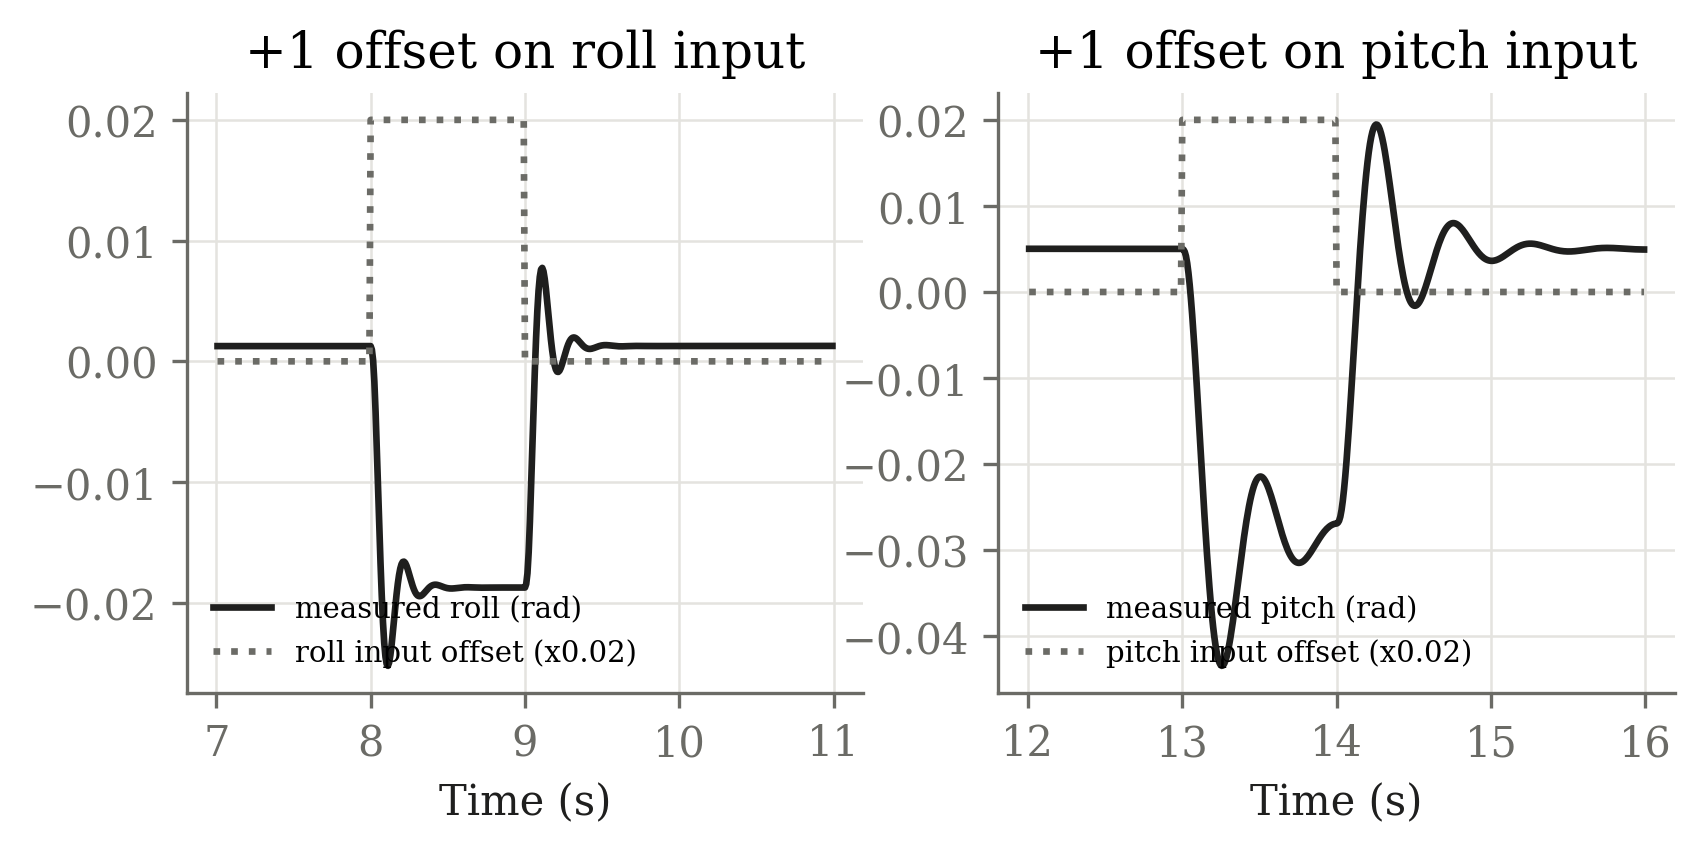
\includegraphics[width=0.92\linewidth]{fig_probe_signs.png}
\caption{Sign probe: response of roll and pitch to a +1 offset on each input}
\label{fig:probe}
\end{figure}

\subsection{Software architecture}
The controller is a Python package with one responsibility per file. Each file has a named owner and its own unit tests (56 tests in total). Table~\ref{tab:files} maps the files to the five team modules.

\begin{table}[h]
\centering
\caption{Software modules and ownership}
\label{tab:files}
\begin{tabular}{|c|P{4.2cm}|P{8cm}|}
\hline
\textbf{Slot} & \textbf{Module} & \textbf{Files} \\ \hline
M1 & State estimation, infrastructure & \texttt{config.py}, \texttt{sensors.py}, \texttt{logger.py}, worlds, sign probe \\ \hline
M2 & Altitude and attitude control & \texttt{pid.py}, \texttt{altitude.py}, \texttt{attitude.py}, \texttt{mixer.py} \\ \hline
M3 & Navigation and trajectory & \texttt{position.py}, \texttt{yaw.py}, \texttt{waypoints.py}, \texttt{trajectory.py} \\ \hline
M4 & Integration and disturbance & \texttt{drone\_main.py}, \texttt{baseline.py}, \texttt{improved.py}, \texttt{wind\_supervisor.py}, \texttt{demo.py} \\ \hline
M5 & Experiments and analysis & \texttt{run\_experiments.py}, \texttt{tune.py}, \texttt{metrics.py}, \texttt{plots.py}, \texttt{tables.py} \\ \hline
\end{tabular}
\end{table}
